\documentclass[10pt,xcolor={dvipsnames}]{beamer}
\usetheme[
%%% option passed to the outer theme
%    progressstyle=fixedCircCnt,   % fixedCircCnt, movingCircCnt (moving is deault)
  ]{Feather}
  
% If you want to change the colors of the various elements in the theme, edit and uncomment the following lines

% Change the bar colors:
\setbeamercolor{Feather}{fg=NavyBlue!20,bg=NavyBlue}

% Change the color of the structural elements:
\setbeamercolor{structure}{fg=NavyBlue}

% Change the frame title text color:
\setbeamercolor{frametitle}{fg=black!5}

% Change the normal text colors:
\setbeamercolor{normal text}{fg=black!75,bg=gray!5}

%% Change the block title colors
\setbeamercolor{block title}{use=Feather,bg=Feather.fg, fg=black!90} 


% Change the logo in the upper right circle:
%\renewcommand{\logofile}{example-grid-100x100pt} 
%% This is an image that comes with the LaTeX installation
% Adjust scale of the logo w.r.t. the circle; default is 0.875
% \renewcommand{\logoscale}{0.55}

% Change the background image on the title and final page.
% It stretches to fill the entire frame!
% \renewcommand{\backgroundfile}{example-grid-100x100pt}

%-------------------------------------------------------
% INCLUDE PACKAGES
%-------------------------------------------------------

\usepackage[utf8]{inputenc}
%\usepackage[english]{babel}
\usepackage[ngerman]{babel}
\usepackage[T1]{fontenc}
% \usepackage{helvet}
\usepackage{svg}
\usepackage{todonotes}

%% Load different font packages to use different fonts
%% e.g. using Linux Libertine, Linux Biolinum and Inconsolata
% \usepackage{libertine}
% \usepackage{zi4}

%% e.g. using Carlito and Caladea
\usepackage{carlito}
\usepackage{caladea}
\usepackage{zi4}

%% e.g. using Venturis ADF Serif and Sans
% \usepackage{venturis}

%-------------------------------------------------------
% DEFFINING AND REDEFINING COMMANDS
%-------------------------------------------------------

% colored hyperlinks
\newcommand{\chref}[2]{
  \href{#1}{{\usebeamercolor[bg]{Feather}#2}}
}

%-------------------------------------------------------
% INFORMATION IN THE TITLE PAGE
%-------------------------------------------------------

\title[] % [] is optional - is placed on the bottom of the sidebar on every slide
{ % is placed on the title page
      \textbf{Grundideen der \strukt}
}

\subtitle[Grundideen der \strukt]
{
      \textbf{Ein Interpretatationsansatz für \bso}
}

\author[Bärbel Hanle]
{      Bärbel Hanle \\
      {\ttfamily bh63mate@studserv.de}\\[1em]
}

\institute[]
{%
      Fakultät für Mathematik und Informatik\\
      Universität Leipzig
}

\date{\today}


%-------------------------------------------------------
% my own commands
%-------------------------------------------------------
% \newcommand{\strukt}{\ensuremath{\mathcal{R}}-Struktur}
% \newcommand{\bs}{\ensuremath{\mathcal{BS}}}
% \newcommand{\bso}{\ensuremath{$\mathcal{BS^O}$}}
% \newcommand{\R}{\ensuremath{$\mathbb{R}$}}

\newcommand{\strukt}{$\mathcal{R}$-Struktur}
\newcommand{\bs}{$\mathcal{BS}$}
\newcommand{\bso}{$\mathcal{BS^O}$}
\newcommand{\R}{\ensuremath{\mathbb{R}}}
\newcommand{\GOrd}{\ensuremath{\mathit{Ord}}}
\newcommand{\GExOrd}{\ensuremath{\mathit{ExOrd}}}
\newcommand{\Geqdim}{\ensuremath{\mathit{eqdim}}}
\newcommand{\Gspart}{\ensuremath{\mathit{spart}}}
\newcommand{\Gscoinc}{\ensuremath{\mathit{scoinc}}}
\newcommand{\Gsov}{\ensuremath{\mathit{sov}}}
\newcommand{\Gsum}{\ensuremath{\mathit{sum}}}
\newcommand{\GLDE}{\ensuremath{\mathit{LDE}}}
\newcommand{\GSB}{\ensuremath{\mathit{SB}}}


%-------------------------------------------------------
% THE BODY OF THE PRESENTATION
%-------------------------------------------------------

\begin{document}

%-------------------------------------------------------
% THE TITLEPAGE
%-------------------------------------------------------

{\1% % this is the name of the PDF file for the background
\begin{frame}[plain,noframenumbering] % the plain option removes the header from the title page, noframenumbering removes the numbering of this frame only
  \titlepage % call the title page information from above
\end{frame}}


\begin{frame}{Überblick}
    Die \strukt\ ist der Versuch, ein Modell für die Theorie \bso\ der ordinären Entitäten des Brentanoraumes zu konstruieren.
    \\ \ \\
    Durch Abschluss unter Summenbildung lässt sich aus dieser Struktur  möglicherweise ein Modell für \bs\ bauen.
    \\ \ \\
    In diesem Vortrag stelle ich die Grundideen dieser Struktur vor.
    Auf die konkrete Umsetzung dieser Ideen werde ich hier nicht eingehen.
%     \\ \ \\
%     Er baut auf Ideen auf, die ich im Rahmen meiner Bachelorarbeit entwickelt habe, weicht aber teilweise davon ab.
%     \\ \ \\
%     Diese Abweichungen sind in den Folien \textcolor{red}{rot} hervorgehoben.
\end{frame}


\begin{frame}{Überblick}{Inhalt}
    \tableofcontents
\end{frame}

%-------------------------------------------------------
\section{Der Brentanoraum}
%-------------------------------------------------------
\subsection{Die Axiomatisierung \bs\ des Brentanoraumes}
%-------------------------------------------------------

%\begin{frame}{Die Axiomatisierung \bs\ des Brentanoraumes}{Erinnerung}
\begin{frame}{\bs}{Erinnerung}
    Die Theorie \bs\ baut auf vier primitive Relationen auf, von denen\\
    \vspace{4pt}
    \begin{tabular}{ r c l }
        $\Gspart(x,y)$ & ... & $x$ ist räumlicher Teil von $y$ und\\
        $\Gscoinc(x,y)$ & ... & $x$ und $y$ koinzidieren
    \end{tabular}\\
    \vspace{4pt}
    für die folgenden Folien relevant sind.
    \\ \ \\
    Was definierte Relationen angeht möchte ich an\\
    \vspace{4pt}
    \begin{tabular}{ r c l }
        $\Geqdim(x,y)$ & ... & $x$ und $y$ sind gleichdimensional,\\
        $\Gsov(x,y)$ & ... & $x$ und $y$ überlappen,\\
        $\Gsum(x,y,z)$ & ... & $z$ ist die mereologische Summe von $x$ und $y$,\\
        $\GLDE(x)$ & ... & $x$ ist eine niederdimensionale Raumentität und\\
        $\GSB(x)$ & ... & $x$ ist eine räumliche Grenze
    \end{tabular}\\
    \vspace{4pt}
    erinnern.
\end{frame}


%\begin{frame}{Die Axiomatisierung \bs\ des Brentanoraumes}{Erinnerung}
\begin{frame}{\bs}{Erinnerung}
    Ganz besonders muss an dieser Stelle die Definition D22 für extraordinäre Raumentitäten
    \begin{align*}
        \GExOrd(x) := \exists yz\ (\Gspart(y,x) \wedge \Gspart(z,x) \wedge \neg\Gsov(y,z) \wedge \Gscoinc(y,z))
    \end{align*}
    hervorgehoben werden.
    \\ \ \\
    Unter den Axiomen ist vor allem A16 relevant, das die uneingeschränkte Existenz der mereologische Summe für gleichdimensionale Raumentitäten fordert.
    \begin{align*}
        \Geqdim(x,y) \to \exists z\ \Gsum(x,y,z)
    \end{align*}
    A33 erlaubt es aus der Ordinärität einer niederdimensionalen Raumentität darauf zu schließen, dass sie eine räumliche Grenze ist
    \begin{align*}
        \GLDE(x) \wedge \GOrd(x) \to \GSB(x)
    \end{align*}
\end{frame}


%-------------------------------------------------------
\subsection{Die Theorie \bso\ der ordinären Entitäten}
%-------------------------------------------------------

% \begin{frame}{Die Theorie \bso\ der ordinären Entitäten}{Allgemeines}
\begin{frame}{\bso}{Allgemeines}
    \begin{itemize}
        \item 
            \bso\ ist die Theorie der ordinären Entitäten des Brentanoraumes.
        \item 
            Sie entsteht aus \bs\ durch Hinzunahme des Axioms
            \begin{align*}
                \text{A0. } \quad \GOrd(x)
            \end{align*}
        \item 
            Nach A33 sind damit alle niederdimensionalen Raumentitäten räumliche Grenzen.
        \item
            Da durch Summenbildung extraordinäre Raumentitäten entstehen können, muss A16 eingeschränkt werden.
    \end{itemize}
\end{frame}

% \begin{frame}{Die Theorie \bso\ der ordinären Entitäten}{Zu A16}
\begin{frame}{\bso}{Zu A16}
    \parbox{0.48\textwidth}{
        Die Abbildung zeigt einen problematischen Fall, bei dem durch die Bildung der mereologischen Summe eine extraordinäre Raumentität entstehen würde.
        \\ \ \\
        Dies liegt daran, dass $x$ und $y$ Teile haben, die koinzidieren aber nicht überlappen.
    }
    \hfill\mbox{}\hfill
    \parbox{0.5\textwidth}{
        \begin{center}
            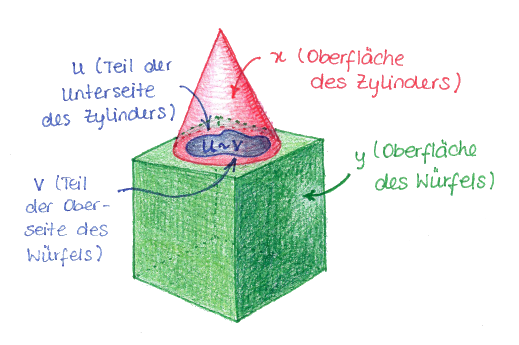
\includegraphics[height=4cm]{img/a16_transparent.png}
        \end{center}
    }\\
    \vspace{8pt}
    Formal ausgedrückt
        \begin{align*}
            \exists uv\ &(\Gspart(u,x) \wedge \Gspart(v,y) \wedge \Gscoinc(u,v) \wedge \neg \Gsov(u,v))
        \end{align*}
\end{frame}


% \begin{frame}{Die Theorie \bso\ der ordinären Entitäten}
%     \parbox{0.5\textwidth}{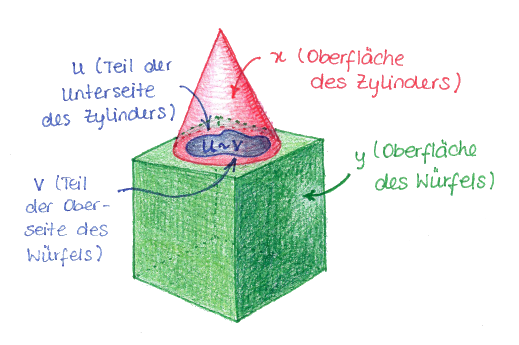
\includegraphics[width=0.5\textwidth]{img/a16_transparent.png}}
%     \parbox{0.38\textwidth}{
%         Dies liegt daran, dass $x$ und $y$ Teile haben, die koinzidieren aber nicht überlappen.\\
%         Formal ausgedrückt
%         \begin{align*}
%             \exists uv\ &(\Gspart(u,x) \wedge \Gspart(v,y)\\
%             &\wedge \Gscoinc(u,v) \wedge \neg \Gsov(u,v))
%         \end{align*}
%     }\\
%     \vspace{8pt}
%     Man beachte, dass diese Formel beinahe der Definition für extraordinäre Raumentitäten entspricht.\\ 
%     Genauer gesagt: Wenn $x$ und $y$ gleich wären, dann würde sie besagen, dass $x$ (und somit $y$) eine extraordinäre Raumentität ist.
% \end{frame}


% \begin{frame}{Die Theorie \bso\ der ordinären Entitäten}{Zu A16}
\begin{frame}{\bso}{Zu A16}
    Die Summe von $x$ und $y$ wird also extraordinär, wenn gilt
    \begin{align*}
        \exists uv\ (\Gspart(u,x) \wedge \Gspart(v,y) \wedge \Gscoinc(u,v) \wedge \neg \Gsov(u,v))
    \end{align*}
    Man beachte, dass diese Formel beinahe der Definition für extraordinäre Raumentitäten entspricht.\\ 
    Genauer gesagt: Wenn $x$ und $y$ gleich wären, dann würde sie besagen, dass $x$ (und somit $y$) eine extraordinäre Raumentität ist.
    \\ \ \\
    Wenn wir diesen Fall ausschließen, ist die Summe von $x$ und $y$ ordinär und kann somit auch in \bso\ existieren.
    A16 muss also modifiziert werden zu
    \begin{align*}
        \text{A16'. }\quad  \neg \exists uv\ (\Gspart(u,x) \wedge \Gspart(v,y) \wedge \Gscoinc(u,v) \wedge \neg \Gsov(u,v))\\
        \mbox{}\wedge \Geqdim(x,y)
        \to \exists z\ \Gsum(x,y,z)
    \end{align*}
\end{frame}


% \begin{frame}{Die Theorie \bso\ der ordinären Entitäten}{Zusammenfassung}
\begin{frame}{\bso}{Zusammenfassung}
    \begin{itemize}
        \item 
            \bso\ ist die Theorie der ordinären Entitäten des Brentanoraumes.
        \item 
            Sie entsteht aus \bs\ durch Hinzunahme des Axioms
            \begin{align*}
                \text{A0. } \quad \GOrd(x)
            \end{align*}
        \item 
            In \bso\ sind alle niederdimensionale Raumentitäten räumliche Grenzen
        \item 
            Damit in \bso\ nicht durch Summenbildung extraordinäre Raumentitäten entstehen, muss A16 eingeschränkt werden zu
            \begin{align*}
                \text{A16'. }\quad  \neg \exists uv\ (\Gspart(u,x) \wedge \Gspart(v,y) \wedge \Gscoinc(u,v) \wedge \neg \Gsov(u,v))\\
                \mbox{}\wedge \Geqdim(x,y)
                \to \exists z\ \Gsum(x,y,z)
            \end{align*}
    \end{itemize}
\end{frame}




%-------------------------------------------------------
\section{Grundideen der \strukt}
%-------------------------------------------------------
\subsection{Euklidische Entitäten}
%-------------------------------------------------------

% \begin{frame}{Euklidische Entitäten}{Allgemeines}
%   \begin{itemize}
%     \item %<1-> 
%         \textbf{Euklidische Entitäten} sind Teilmengen des $\R^3$
%     \item %<2-> 
%         Sie zerfallen in euklidische \textcolor{red}{\textbf{Körper}}%
%         \footnote{
%             nicht zu verwechseln mit dem Begriff des euklidischen Körpers in der Algebra
%         }%
%         , \textbf{Flächen}, \textbf{Linien} und \textbf{Punktmengen}.
%     \item %<3-> 
%         Euklidische Entitäten, die keine euklidischen Punktmengen sind heißen \textcolor{red}{\textbf{höherdimensionale}} euklidische Entitäten.
%     \item %<4-> 
%         Euklidische Entitäten, die keine euklidischen Körper sind heißen \textbf{niederdimensionale} euklidische Entitäten.
%     \item %<5-> 
%         Höherdimensionale euklidische Entitäten haben einen Rand.%
%         \footnote{
%             Dieser kann sich vom Rand im topologischen Sinn unterscheiden
%         }
%   \end{itemize}
% \end{frame}


\begin{frame}{Euklidische Entitäten}{Allgemeines}
  \begin{itemize}
    \item %<1-> 
        \textbf{Euklidische Entitäten} sind Teilmengen des $\R^3$
    \item %<2-> 
        Sie zerfallen in \textbf{Raumregionen}, \textbf{euklidische Flächen}, \textbf{euklidische Linien} und \textbf{euklidische Punktmengen}.
    \item %<3-> 
        Euklidische Entitäten, die keine euklidischen Punktmengen sind heißen höherdimensionale euklidische Entitäten.
    \item %<4-> 
        Euklidische Entitäten, die keine Raumregionen sind heißen \textbf{niederdimensionale} euklidische Entitäten.
    \item %<5-> 
        Höherdimensionale euklidische Entitäten haben einen Rand.%
        \footnote{
            Dieser kann sich vom Rand im topologischen Sinn unterscheiden
        }
  \end{itemize}
\end{frame}


% \begin{frame}{Euklidische Entitäten}{Euklidische Körper, Flächen, Linien und Punktmengen}
%     Niederdimensionale euklidische Entitäten sind bestimmte Teilmengen des Randes von höherdimensionalen.\\ \ \\
%     Konkret bedeutet dies:
%     \begin{itemize}
%         \item Eine euklidische Fläche ist eine Teilmenge des Randes eines euklidischen Körpers, die bestimmte Eigenschaften erfüllt.
%         \item Eine euklidische Linie ist eine Teilmenge des Randes einer euklidischen Fläche, die bestimmte Eigenschaften erfüllt.
%         \item Eine euklidische Punktmenge ist eine Teilmenge des Randes einer euklidischen Linie.
%         \footnote{
%             Im vorgeschlagenen Ansatz muss eine euklidische Punktmenge keine weiteren Bedingungen erfüllen. Dies ist im Rahmen der Grundidee aber durchaus denkbar.
%         }
%     \end{itemize}
%      %
%     \begin{tikzpicture}[overlay,shift={(current page.center)}]
%         \node at (2.7cm,-3.8cm) {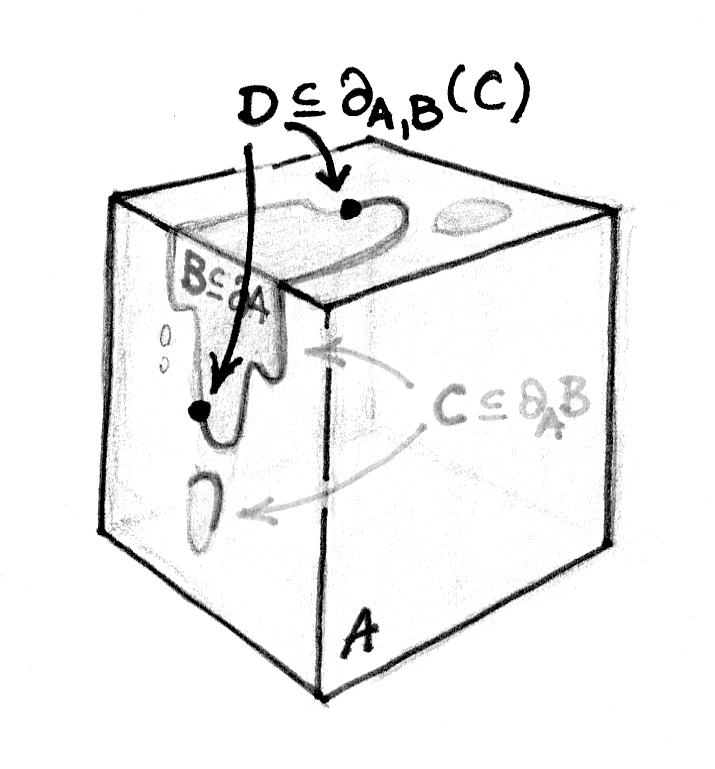
\includegraphics[height=3.6cm]{img/eukl-entit_transparent.png}};
%     \end{tikzpicture}
% \end{frame}


% \begin{frame}{Euklidische Entitäten}{Euklidische Körper, Flächen, Linien und Punktmengen}
%     Niederdimensionale euklidische Entitäten sind bestimmte Teilmengen des Randes von höherdimensionalen.\\ \ \\
%     Konkret bedeutet dies:
%     %\begin{block}{Euklidische Körper, Flächen, Linien und Punktmengen}
%         \begin{itemize}
%         \item Eine euklidische Fläche ist eine Teilmenge des Randes eines euklidischen Körpers, die bestimmte Eigenschaften erfüllt.
%         \item Eine euklidische Linie ist eine Teilmenge des Randes einer euklidischen Fläche, die bestimmte Eigenschaften erfüllt.
%         \item Eine euklidische Punktmenge ist eine Teilmenge des Randes einer euklidischen Linie.
%         \footnote{
%             Im vorgeschlagenen Ansatz muss eine euklidische Punktmenge keine weiteren Bedingungen erfüllen. Dies ist im Rahmen der Grundidee aber durchaus denkbar.
%         }
%       \end{itemize}
% \end{frame}


\begin{frame}{Euklidische Entitäten}{Raumregionen, Flächen, Linien und Punktmengen}
    Niederdimensionale euklidische Entitäten sind bestimmte Teilmengen des Randes von höherdimensionalen.\\ \ \\
    Konkret bedeutet dies:
        \begin{itemize}
        \item Eine euklidische Fläche ist eine Teilmenge des Randes einer Raumregion, die bestimmte Eigenschaften erfüllt.
        \item Eine euklidische Linie ist eine Teilmenge des Randes einer euklidischen Fläche, die bestimmte Eigenschaften erfüllt.
        \item Eine euklidische Punktmenge ist eine Teilmenge des Randes einer euklidischen Linie, die bestimmte Bedingungen erfüllt.
      \end{itemize}
\end{frame}


% \begin{frame}{Euklidische Entitäten}{Beispiel}
%     \begin{itemize}
%         \item $A$ ist ein euklidischer Körper.
%         \item $B$ ist eine euklidische Fläche.
%         \item $C$ ist eine euklidische Linie.
%         \item $D$ ist eine euklidische Punktmenge.
%     \end{itemize}
%     \begin{tikzpicture}[overlay,shift={(current page.center)}]
%         \node at (2.7cm,-3.8cm) {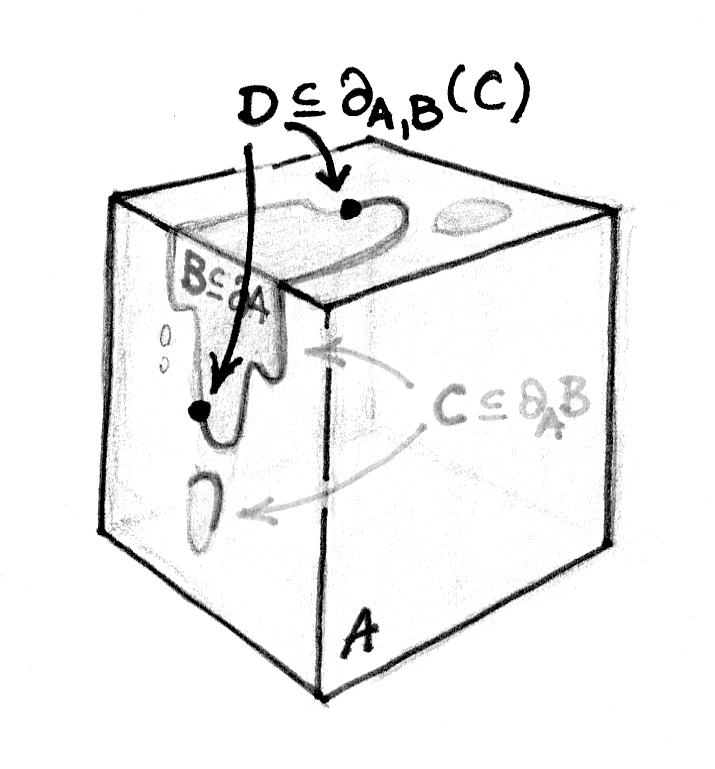
\includegraphics[height=3.6cm]{img/eukl-entit_transparent.png}};
%     \end{tikzpicture}
% \end{frame}


\begin{frame}{Euklidische Entitäten}{Beispiel}
    \begin{itemize}
        \item $A$ ist eine Raumregion.
        \item $B$ ist eine euklidische Fläche.
        \item $C$ ist eine euklidische Linie.
        \item $D$ ist eine euklidische Punktmenge.
    \end{itemize}
    \begin{tikzpicture}[overlay,shift={(current page.center)}]
        \node at (2.7cm,-3.8cm) {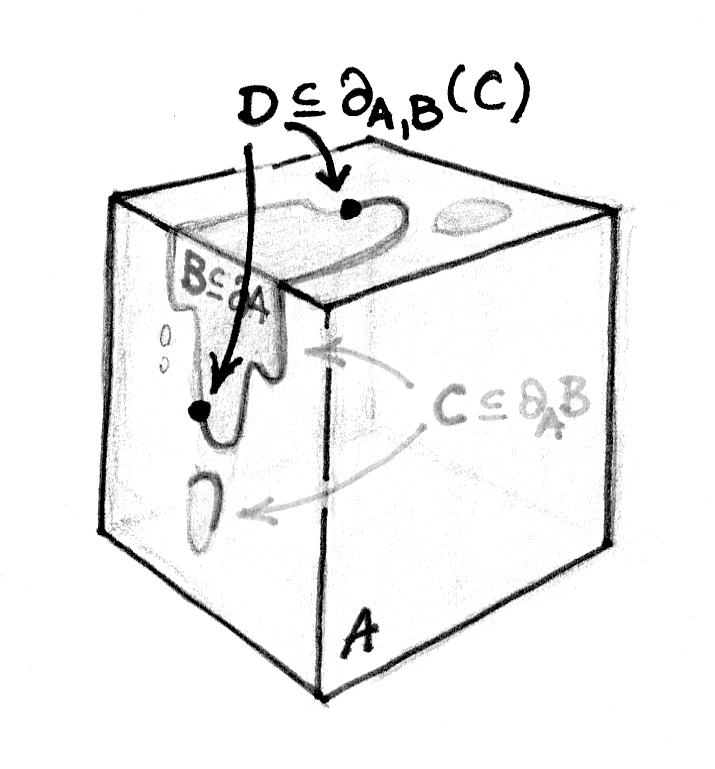
\includegraphics[height=3.6cm]{img/eukl-entit_transparent.png}};
    \end{tikzpicture}
\end{frame}


% \begin{frame}{Euklidische Entitäten}{euklidische Körper}
% \parbox{0.7\textwidth}{
%         Wenn wir davon ausgehen, dass der Raum, den das Universum einnimmt mit dem $\R^3$ identifizieren lässt, entsprechen die euklidischen Entitäten den Teilmengen des $\R^3$, die von materiellen Körpern eingenommen werden können.
%     }
%     \hfill\mbox{}\hfill
%     \parbox{0.25\textwidth}{
%         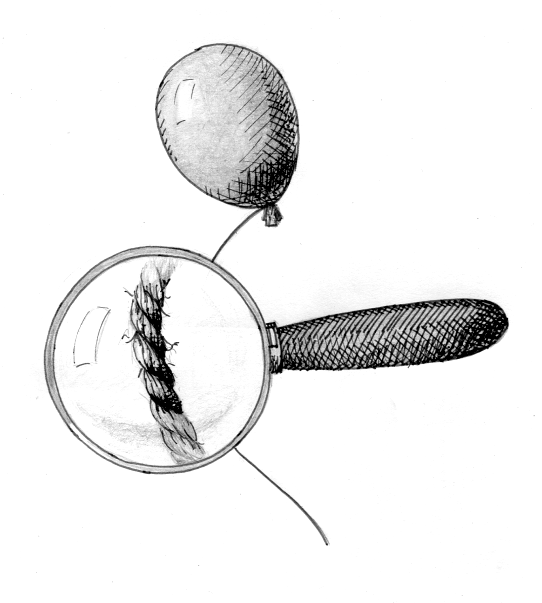
\includegraphics[height=3cm]{img/echt-3-dim-transparent.png}
%     }
%     \begin{block}{Eigenschaften euklidischer Körper}
%         \begin{itemize}
%             \item Euklidische Körper sind überall echt 3-dimensional.
%             \item Ihr Rand ist überall echt 2-dimensional.
%             \item Sie besitzen keine niederdimensionalen Löcher.
%         \end{itemize}
%     \end{block}
% \end{frame}


% \begin{frame}{Euklidische Entitäten}{Euklidische Körper}
%     Wenn wir davon ausgehen, dass der Raum, den das Universum einnimmt mit dem $\R^3$ identifizieren lässt, entsprechen die euklidischen Körper den Teilmengen des $\R^3$, die von materiellen Körpern eingenommen werden können.\\ \ \\
%     Diese haben folgende Eigenschaften
%     \begin{itemize}
%         \item Euklidische Körper sind überall echt 3-dimensional.
%         \item Ihr Rand ist überall echt 2-dimensional.
%         \item Sie besitzen keine niederdimensionalen Löcher.
%     \end{itemize}
%     %
%     \begin{tikzpicture}[overlay,shift={(current page.center)}]
%         \node at (2.7cm,-4.7cm) {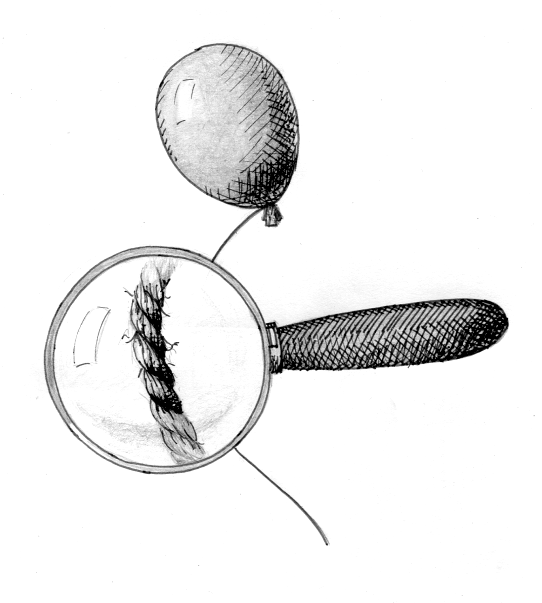
\includegraphics[height=3.6cm]{img/echt-3-dim-transparent.png}};
%     \end{tikzpicture}
% \end{frame}


\begin{frame}{Euklidische Entitäten}{Raumregionen}
    Wenn wir davon ausgehen, dass der Raum, den das Universum einnimmt mit dem $\R^3$ identifizieren lässt, entsprechen die Raumregionen den Teilmengen des $\R^3$, die von materiellen Körpern eingenommen werden können.\\ \ \\
    Diese haben folgende Eigenschaften
    \begin{itemize}
        \item Sie sind überall echt $3$-dimensional.
        \item Ihr Rand ist überall echt $2$-dimensional.
        \item Sie besitzen keine niederdimensionalen Löcher.
        \item Sie sind beschränkt.
    \end{itemize}
    %
    \begin{tikzpicture}[overlay,shift={(current page.center)}]
        \node at (2.7cm,-4.3cm) {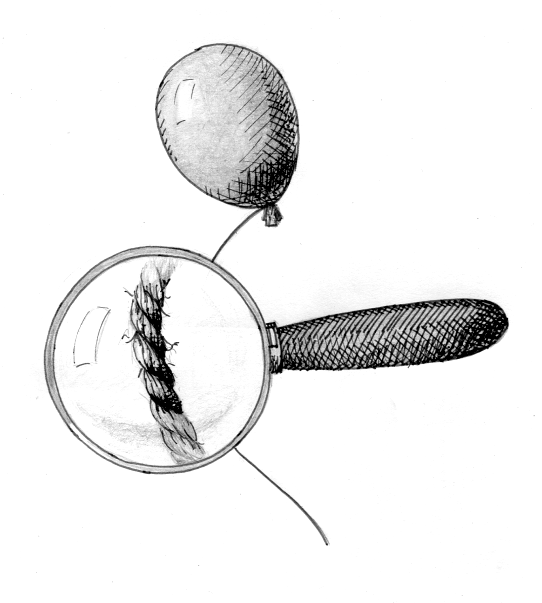
\includegraphics[height=3.6cm]{img/echt-3-dim-transparent.png}};
    \end{tikzpicture}
\end{frame}


% \begin{frame}{Euklidische Entitäten}{Niederdimensionale euklidische Entitäten}
%     Niederdimensionale euklidische Entitäten lassen sich als Teilmengen des Randes von höherdimensionalen konstruieren.\\ \ \\
%     Genauer gesagt: 
%     %
%     \begin{itemize}
%         \item Eine \textbf{euklidische Fläche} ist eine Teilmenge des Randes eines euklidischen Körpers.
%             Ihr Rand ist überall echt 1-dimensional und sie besitzen keine $1$- oder $0$-dimensionalen Löcher.
%         \item Eine \textbf{euklidische Linie} ist eine Teilmenge des Randes einer euklidischen Fläche.
%             Ihr Rand ist überall echt $0$-dimensional und sie besitzen keine $0$-dimensionalen Löcher.
%         \item Eine \textbf{euklidische Punktmenge} ist eine Teilmenge des Randes einer euklidischen Linie.
%     \end{itemize}
% \end{frame}


\begin{frame}{Euklidische Entitäten}{Niederdimensionale euklidische Entitäten}
    Niederdimensionale euklidische Entitäten lassen sich als Teilmengen des Randes von höherdimensionalen konstruieren.\\ \ \\
    Genauer gesagt: 
    %
    \begin{itemize}
        \item Eine \textbf{euklidische Fläche} ist eine Teilmenge des Randes einer Raumregion.
            Ihr Rand ist überall echt $1$-dimensional und sie besitzen keine $1$- oder $0$-dimensionalen Löcher.
        \item Eine \textbf{euklidische Linie} ist eine Teilmenge des Randes einer euklidischen Fläche.
            Ihr Rand ist überall echt $0$-dimensional und sie besitzen keine $0$-dimensionalen Löcher.
        \item Eine \textbf{euklidische Punktmenge} ist eine Teilmenge des Randes einer euklidischen Linie.
    \end{itemize}
\end{frame}


% \begin{frame}{Euklidische Entitäten}{Niederdimensionale euklidische Entitäten}
%     Niederdimensionale euklidische Entitäten lassen sich als Teilmengen des Randes von höherdimensionalen konstruieren.\\ \ \\
%     Genauer gesagt: 
%     %
%     \begin{itemize}
%         \item Eine \textbf{euklidische Fläche} ist eine Teilmenge des Randes eines euklidischen Körpers.
%             Ihr Rand ist überall echt 1-dimensional und sie besitzen keine $1$- oder $0$-dimensionalen Löcher.
%         \item Eine \textbf{euklidische Linie} ist eine Teilmenge des Randes\\ 
%             einer euklidischen Fläche.
%             Ihr Rand ist überall\\
%             echt $0$-dimensional und sie besitzen keine $0$-\\
%             dimensionalen Löcher.
%         \item Eine \textbf{euklidische Punktmenge} ist eine Teil-\\menge des Randes einer euklidischen Linie.
%     \end{itemize}
%     %
%     \begin{tikzpicture}[overlay,shift={(current page.center)}]
%         \node at (2.7cm,-3.8cm) {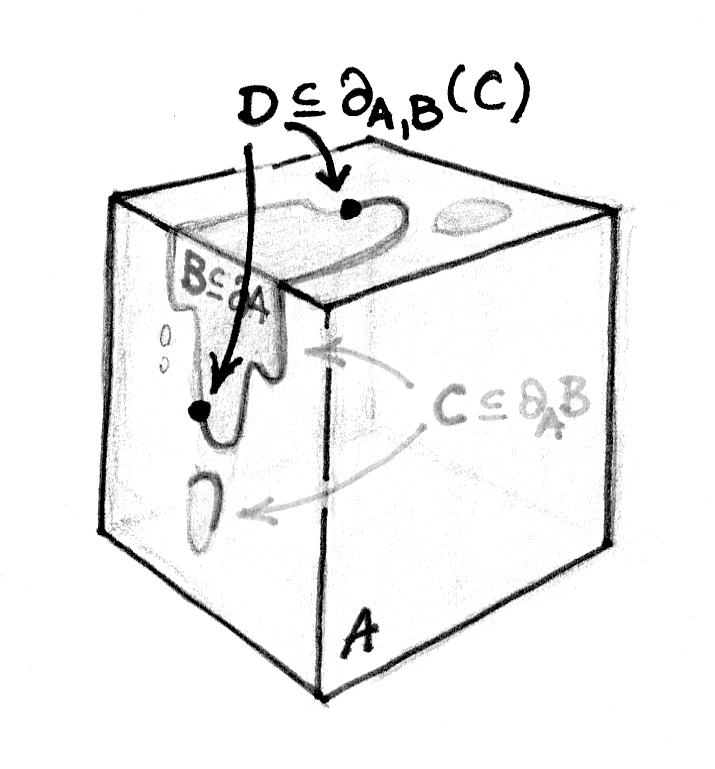
\includegraphics[height=3.6cm]{img/eukl-entit_transparent.png}};
%     \end{tikzpicture}
% \end{frame}

%-----------------------------------------------------------------
\subsection{Repräsentanten}
%-----------------------------------------------------------------

% \begin{frame}{Repräsentanten}{Allgemeines}
%     Zu jeder euklidischen Punktmenge gehören bestimmte euklidische Linien, zu denen bestimmte euklidischen Flächen gehören, zu denen bestimmte euklidische Körper gehören.\\ \ \\
%     Tupel aus zusammengehörigen euklidischen Entitäten sind \textbf{Repräsentanten} der Individuen der \strukt.
%     \begin{tikzpicture}[overlay,shift={(current page.center)}]
%         \node at (-9.5cm,-5.5cm) {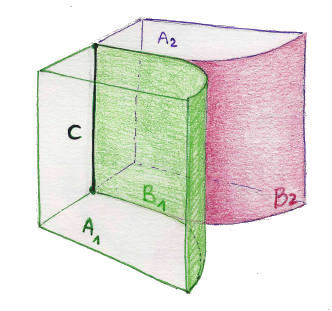
\includegraphics[height=3.5cm]{img/spart-linien_transparent.png}};
%     \end{tikzpicture}
% \end{frame}

% \begin{frame}{Repräsentanten}{Allgemeines}
%     Zu jeder euklidischen Punktmenge gehören bestimmte euklidische Linien, zu denen bestimmte euklidischen Flächen gehören, zu denen bestimmte euklidische Körper gehören.\\ \ \\
%     Tupel aus zusammengehörigen euklidischen Entitäten sind \textbf{Repräsentanten} der Individuen der \strukt.\\
%     \vspace{0.5cm}
%     \parbox{0.3\textwidth}{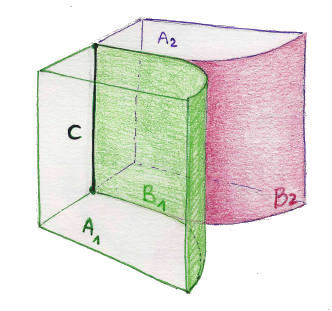
\includegraphics[height=3.5cm]{img/spart-linien_transparent.png}}
%     \hfill\mbox{}\hfill
%     \parbox{0.6\textwidth}{Zu $C$ gehören sowohl $B_1$ als auch $B_2$ als euklidische Flächen, während unter den dargestellten euklidischen Körpern nur $A_1$ zu $B_1$ gehört und nur $A_2$ zu $B_2$.}
% \end{frame}


% \begin{frame}{Repräsentanten}{Vorbemerkungen}
%     \parbox{0.2\textwidth}{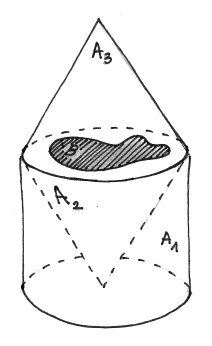
\includegraphics[height=3.5cm]{img/objektaeq-flaechen_transparent.png}}
%     \hfill\mbox{}\hfill
%     \parbox{0.7\textwidth}{
%         Zu jeder euklidischen Punktmenge gehören bestimmte euklidische Linien, zu denen bestimmte euklidischen Flächen gehören, zu denen bestimmte euklidische Körper gehören.\\ \ \\
%         In der Abbildung gehören $A_1$, $A_2$ und $A_3$ als euklidische Körper alle zur euklidischen Fläche B.
%     }
% \end{frame}


\begin{frame}{Repräsentanten}{Vorbemerkungen}
    \parbox{0.2\textwidth}{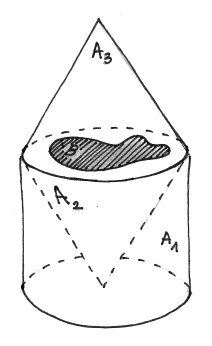
\includegraphics[height=3.5cm]{img/objektaeq-flaechen_transparent.png}}
    \hfill\mbox{}\hfill
    \parbox{0.7\textwidth}{
        Zu jeder euklidischen Punktmenge gehören bestimmte euklidische Linien, zu denen bestimmte euklidischen Flächen gehören, zu denen bestimmte Raumregionen gehören.\\ \ \\
        In der Abbildung gehören $A_1$, $A_2$ und $A_3$ als euklidische Körper alle zur euklidischen Fläche $B$.
    }
\end{frame}


\begin{frame}{Repräsentanten}{Flächen-, Linien- und Punktrepräsentanten}
    Tupel aus zusammengehörigen euklidischen Entitäten sind \textbf{Repräsentanten} der Individuen der \strukt.\\ \ \\
    Je nach Tupellänge werden dabei drei Arten von Repräsentanten unterschieden:
    %
    \begin{enumerate}
        \item \textbf{Flächenrepräsentanten}
            sind Paare aus einer Raumregion und einer euklidischen Fläche auf ihrem Rand.
        \item \textbf{Linienrepräsentanten}
            sind Tripel aus einer Raumregion, einer euklidischen Fläche auf ihrem Rand und einer euklidischen Linie auf deren Rand.
        \item \textbf{Punktrepräsentanten}
            sind Quadrupel aus einer Raumregion, einer euklidischen Fläche auf ihrem Rand, einer euklidischen Linie auf deren Rand und einer euklidischen Punktmenge auf dem Rand der Linie.%
    \end{enumerate}
\end{frame}


\begin{frame}{Repräsentanten}{Beispiel}
    \begin{itemize}
        \item $(A,B)$ ist ein Flächenrepräsentant.
        \item $(A,B,C)$ ist ein Linienrepräsentant.
        \item $(A,B,C,D)$ ist ein Punktrepräsentant.
    \end{itemize}
        %
    \begin{tikzpicture}[overlay,shift={(current page.center)}]
        \node at (2cm,-5cm) {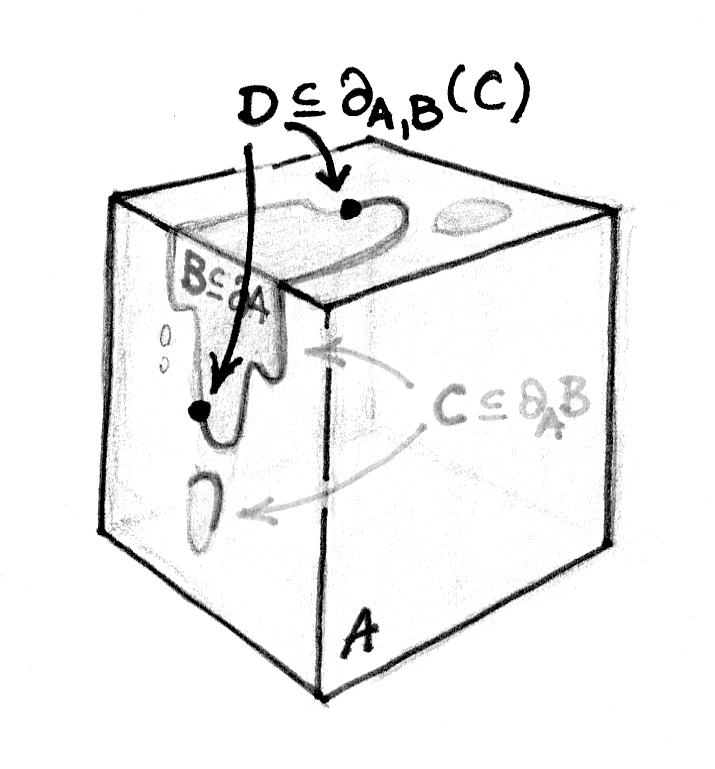
\includegraphics[height=5cm]{img/eukl-entit_transparent.png}};
    \end{tikzpicture}
\end{frame}


%-----------------------------------------------------------------
\subsection{Objektäquivalenz}
%-----------------------------------------------------------------

% \begin{frame}{Objektäquivalenz}{Motivation}
%     Im Rahmen der \bso-Theorie können verschiedene Repräsentanten die gleiche Raumentität repräsentieren.\\
%     %\vspace{1cm}
%     \parbox{0.2\textwidth}{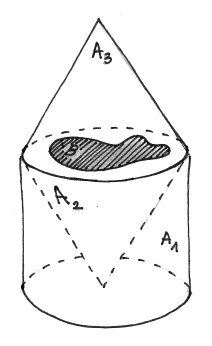
\includegraphics[height=2.8cm]{img/objektaeq-flaechen_transparent.png}}
%     \parbox{0.75\textwidth}{
%         In der linken Abbildung repräsentieren $(A_1,B)$ und $(A_2,B)$ die selbe Flächenregion, $(A_3,B)$ eine andere.\\ \ \\
%         Das liegt daran, dass $A_1$ und $A_2$ \glqq von unten\grqq\ auf $B$ zukommen, $A_3$ \glqq von oben\grqq.
%     }
%     \parbox{0.7\textwidth}{Bei Linienrepräsentanten stellt sich die Situation komplizierter dar, da hier nicht nur die euklidischen Flächen, sondern auch die zugehörigen euklidischen Körper von der gleichen Seite kommen müssen.\\ \ \\
%     In der rechten Abbildung repräsentieren $(A_1,B_1,C)$ deshalb nicht die gleiche Linienregion wie $(A_2,B_2,C)$.}
%     \parbox{0.25\textwidth}{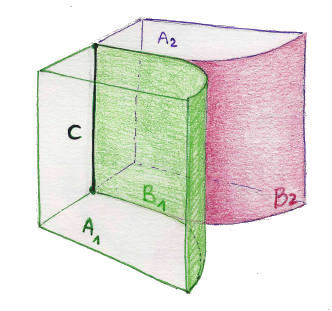
\includegraphics[height=3cm]{img/spart-linien_transparent.png}}
% \end{frame}

% \begin{frame}{Objektäquivalenz}
%     Die \textbf{Objektäquivalenz} ist eine Äquivalenzrelation auf der Menge der niederdimensionalen euklidischen Entitäten, die dieses \glqq in allen Dimensionen von der gleichen Seite kommen\grqq\ in geeigneter Weise erfasst.
% \end{frame}

\begin{frame}{Objektäquivalenz}{Motivation}
    Im Rahmen der \bso-Theorie können verschiedene Repräsentanten die gleiche Raumentität repräsentieren.\\
    \vspace{1cm}
    \parbox{0.2\textwidth}{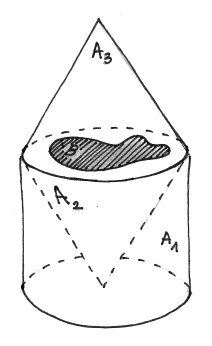
\includegraphics[height=2.8cm]{img/objektaeq-flaechen_transparent.png}}
    \parbox{0.75\textwidth}{
        In der linken Abbildung repräsentieren $(A_1,B)$ und $(A_2,B)$ die selbe Flächenregion, $(A_3,B)$ eine andere.\\ \ \\
        Das liegt daran, dass $A_1$ und $A_2$ \glqq von unten\grqq\ auf $B$ zukommen, $A_3$ \glqq von oben\grqq.
    }
\end{frame}


% \begin{frame}{Objektäquivalenz}
%     \parbox{0.7\textwidth}{Bei Linienrepräsentanten stellt sich die Situation komplizierter dar, da hier nicht nur die euklidischen Flächen, sondern auch die zugehörigen euklidischen Körper von der gleichen Seite kommen müssen.\\ \ \\
%     In der rechten Abbildung repräsentiert $(A_1,B_1,C)$ deshalb \textit{nicht} die gleiche Linienregion wie $(A_2,B_2,C)$.}
%     \parbox{0.25\textwidth}{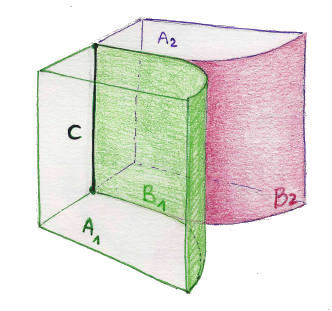
\includegraphics[height=3cm]{img/spart-linien_transparent.png}}
%     \vspace{0.5cm}\\
%     Die \textbf{Objektäquivalenz} ist eine Äquivalenzrelation auf der Menge der niederdimensionalen euklidischen Entitäten, die dieses \glqq in allen Dimensionen von der gleichen Seite kommen\grqq\ in geeigneter Weise erfasst.
% \end{frame}


% \begin{frame}{Objektäquivalenz}{Beispiel}
%     \parbox{0.7\textwidth}{Bei Linienrepräsentanten stellt sich die Situation komplizierter dar, da hier nicht nur die euklidischen Flächen, sondern auch die zugehörigen Raumregionen von der gleichen Seite kommen müssen.\\ \ \\
%     In der rechten Abbildung repräsentiert $(A_1,B_1,C)$ deshalb \textit{nicht} die gleiche Linienregion wie $(A_2,B_2,C)$.}
%     \parbox{0.25\textwidth}{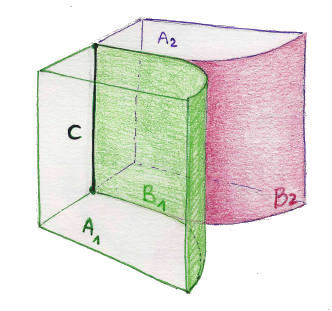
\includegraphics[height=3cm]{img/spart-linien_transparent.png}}
% \end{frame}


\begin{frame}{Objektäquivalenz}{Beispiel}
    Bei Linienrepräsentanten stellt sich die Situation komplizierter dar, da hier nicht nur die euklidischen Flächen, sondern auch die zugehörigen Raumregionen von der gleichen Seite kommen müssen.\\
    \vspace{0.5cm}
    \parbox{0.25\textwidth}{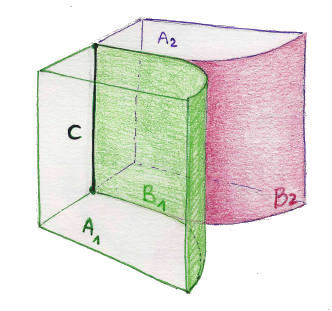
\includegraphics[height=3cm]{img/spart-linien_transparent.png}}
    \hfill\mbox{}\hfill
    \parbox{0.58\textwidth}{
        In der linken Abbildung repräsentiert $(A_1,B_1,C)$ deshalb \textit{nicht} die gleiche Linienregion wie $(A_2,B_2,C)$.
    }
    \hfill\mbox{}\hfill
\end{frame}


% \begin{frame}{Objektäquivalenz}{Diskussion}
%     Was es heißt, dass zwei euklidische Körper von der gleichen Seite auf eine euklidische Fläche zukommen ist auch intuitiv nicht immer einfach zu beantworten.\\
%     \vspace{-10pt}
%     \begin{center}
%         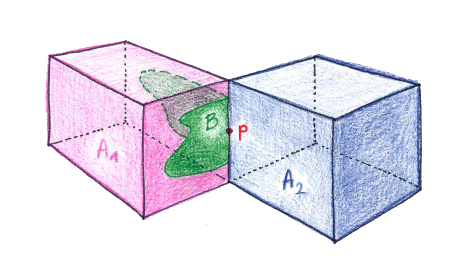
\includegraphics[height=3.5cm]{img/objektaeq_transparent.png}  
%     \end{center}
%     \vspace{-10pt}
%     Sollen $( A_1 , B )$ und $( A_1 \cup A_2 , B )$ äquivalent sein?\\
%     Kommen $A_1$ und $A_1 \cup A_2$ bei $p$ von der gleichen Seite auf $B$ zu?
% \end{frame}


% \begin{frame}{Objektäquivalenz}{Diskussion}
%     Die \textbf{Objektäquivalenz} ist eine Äquivalenzrelation auf der Menge der niederdimensionalen euklidischen Entitäten, die dieses \glqq in allen Dimensionen von der gleichen Seite kommen\grqq\ in geeigneter Weise erfasst.
%     \\ \ \\
%     Was es heißt, dass zwei Raumregionen von der gleichen Seite auf eine euklidische Fläche zukommen ist auch intuitiv nicht immer einfach zu beantworten.\\
%     \vspace{-10pt}
%     \begin{center}
%         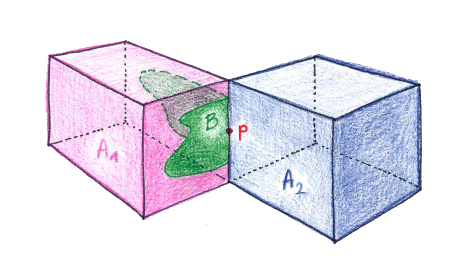
\includegraphics[height=3.5cm]{img/objektaeq_transparent.png}  
%     \end{center}
%     \vspace{-10pt}
%     Sollen $( A_1 , B )$ und $( A_1 \cup A_2 , B )$ äquivalent sein?\\
%     Kommen $A_1$ und $A_1 \cup A_2$ bei $p$ von der gleichen Seite auf $B$ zu?
% \end{frame}


\begin{frame}{Objektäquivalenz}{Definition und Diskussion}
    Die \textbf{Objektäquivalenz} ist eine Äquivalenzrelation auf der Menge der Repräsentanten, die dieses \glqq in allen Dimensionen von der gleichen Seite kommen\grqq\ in geeigneter Weise erfasst.
    \\ \ \\
    Was es heißt, dass zwei Raumregionen von der gleichen Seite auf eine euklidische Fläche zukommen ist auch intuitiv nicht immer einfach zu beantworten.\\
    \parbox{0.5\textwidth}{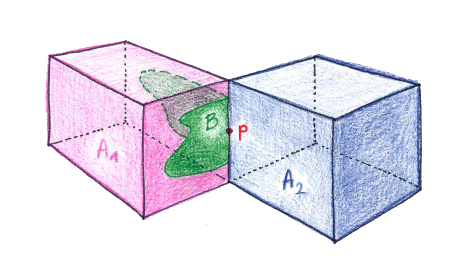
\includegraphics[height=3.5cm]{img/objektaeq_transparent.png}}
    \hfill\mbox{}\hfill
    \parbox{0.4\textwidth}{
        Sollen $( A_1 , B )$ und $( A_1 \cup A_2 , B )$ äquivalent sein?\\
        Kommen $A_1$ und $A_1 \cup A_2$ bei $p$ von der gleichen Seite auf $B$ zu?
    }
    \hfill\mbox{}\hfill
\end{frame}


%-----------------------------------------------------------------
% \subsection{Raumentitäten}
\subsection{Das Universum der \strukt}
%-----------------------------------------------------------------

%\begin{frame}{Raumentitäten}{Niederdimensionale Raumentitäten}
\begin{frame}{Das Universum der \strukt}{Niederdimensionale Raumentitäten}
%     Die niederdimensionalen Entitäten des Brentanoraumes werden in der \strukt\ zu Äquivalenzklassen einer Objektäquivalenz interpretiert.\\
%     Sie heißen Flächen-, Linien- und Punktregionen.
    \begin{block}{Definition}
        Sei $\sim$ ein Objektäquivalenz.
        \begin{enumerate}
            \item 
                Für einen Flächenrepräsentanten $(A,B)$ bezeichnet $[A,B]$ die Äquivalenzklasse bzgl.\ $\sim$.
                Diese Äquivalenzklassen heißen \textbf{Flächenregionen}.
            \item 
                Für einen Linienrepräsentanten $(A,B,C)$ bezeichnet $[A,B,C]$ die Äquivalenzklasse bzgl.\ $\sim$.
                Diese Äquivalenzklassen heißen \textbf{Linienregionen}.
            \item 
                Für einen Punktrepräsentanten $(A,B,C,D)$ bezeichnet $[A,B,C,D]$ die Äquivalenzklasse bzgl.\ $\sim$.
                Diese Äquivalenzklassen heißen \textbf{Punktregionen}.
        \end{enumerate}
    \end{block}
\end{frame}


% \begin{frame}{Raumentitäten}{Beispiel und Universum}
\begin{frame}{Das Universum der \strukt}{Beispiel}
    \parbox{0.3\textwidth}{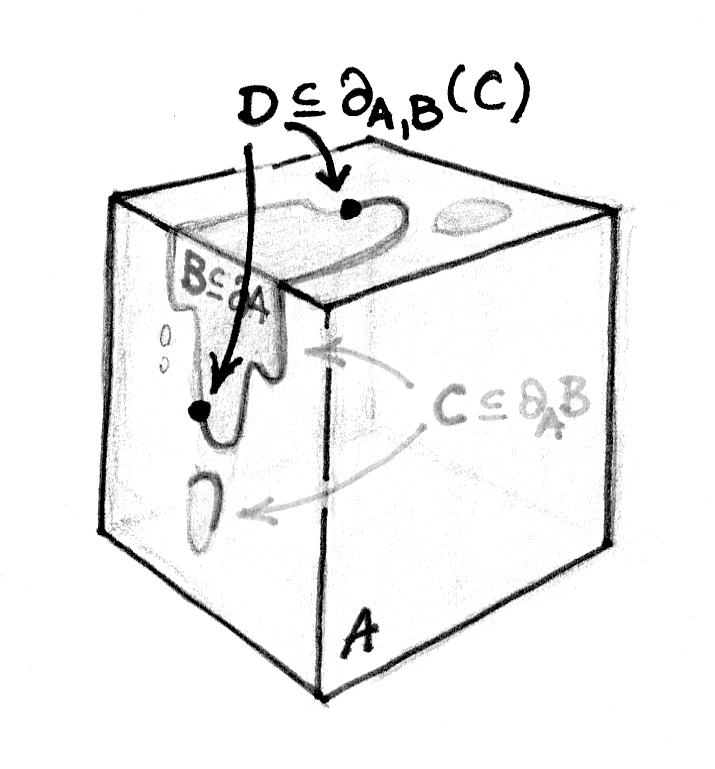
\includegraphics[height=4cm]{img/eukl-entit_transparent.png}}
    \hfill\mbox{}\hfill
    \parbox{0.6\textwidth}{
    In der Abbildung ist
    \begin{itemize}
        \item $A$ eine Raumregion,
        \item $[A,B]$ eine Flächenregion,
        \item $[A,B,C]$ eine Linienregion und
        \item $[A,B,C,D]$ eine Punktregion.
    \end{itemize}
    }
\end{frame}


% % \begin{frame}{Raumentitäten}{Beispiel und Universum}
% \begin{frame}{Das Universum der \strukt}{Definition}
%     Das \textbf{Universum} der \strukt besteht aus den Raum-, Flächen-, Linien- und Punktregionen.
% \end{frame}

% \begin{frame}{Raumentitäten}{Beispiel und Universum}
\begin{frame}{Das Universum der \strukt}{Definition}
\begin{center}
    \includegraphics[width=1\textwidth]{img/universum.png}
\end{center}
\end{frame}

%-----------------------------------------------------------------
\subsection{Primitive Relationen}
%-----------------------------------------------------------------

%-----------------------------------------------------------------
\section{Topologische Definitionen}
%-----------------------------------------------------------------
%-----------------------------------------------------------------
\subsection{Lokale Gleichheit}
%-----------------------------------------------------------------
%-----------------------------------------------------------------
\subsection{Einfache Mengen}
%-----------------------------------------------------------------
%-----------------------------------------------------------------
\subsection{Äußerer Rand}
%-----------------------------------------------------------------

\end{document}
